\providecommand{\tightlist}{%
  \setlength{\itemsep}{0pt}\setlength{\parskip}{0pt}
}
% \def\tightlist{}
% \documentclass[biblatex,ddraft]{deltares_report}
\documentclass[ddraft]{deltares_report}
\begin{document}
\title{Zeespiegelmonitor}
\subtitle{2023-2026}
\author{Stolte, Willem et al.}
% \partner{Partners}

\client{Rijkswaterstaat, Ministerie van Infrastructuur en Watermanagement}
\contact{Saskia van Gool}
\reference{Reference}
\keywords{Zeespiegelstijging, Kustbeleid, Zandsuppletie}

\version{0.1}
\date{}
\projectnumber{123456789}
\documentid{Id}
\status{Concept}
\disclaimer{Disclaimer}
%\references{References}

\authori{Stolte, W.}
\organisationi{Deltares}
\authorii{Lebars, D.}
\organisationii{KNMI}
\versioni{0.9}
\revieweri{Taal, M.}
\approvali{Snippen, E}
\publisheri{Deltares}

\summary{
\lipsum[1]

\lipsum[2]

\lipsum[3]
}
\deltarestitle
%------------------------------------------------------------------------------

% Text body
\bookmarksetup{startatroot}

\chapter*{Preface}\label{preface}
\addcontentsline{toc}{chapter}{Preface}

\markboth{Preface}{Preface}

\section*{Lijst met afkortingen}\label{lijst-met-afkortingen}
\addcontentsline{toc}{section}{Lijst met afkortingen}

\markright{Lijst met afkortingen}

\begin{description}
\tightlist
\item[\phantomsection\label{acronyms_20CR}{20CR}]
20th Century (Climate) Reanalysis
\item[\phantomsection\label{acronyms_AGRS}{AGRS}]
Actief GNSS Referentie Systeem
\item[\phantomsection\label{acronyms_AHN}{AHN}]
Actueel Hoogtebestand Nederland
\item[\phantomsection\label{acronyms_AIC}{AIC}]
Akaike Informatie Criterium, (een maat voor de goodness-of-fit van een
model)
\item[\phantomsection\label{acronyms_AMO}{AMO}]
Atlantic Multidecadal Oscillation
\item[\phantomsection\label{acronyms_AR}{AR}]
Autoregressie
\item[\phantomsection\label{acronyms_AR5}{AR5}]
Fifth Assessment Report IPCC
\item[\phantomsection\label{acronyms_AVISO}{AVISO}]
Archiving, Validation and Interpretation of Satellite Oceanographic data
\item[\phantomsection\label{acronyms_Argo}{Argo}]
Argo, vernoemd naar schip uit de Griekse mythologie
\item[\phantomsection\label{acronyms_BGT}{BGT}]
Basisregistratie Grootschalige Topografie
\item[\phantomsection\label{acronyms_BKL}{BKL}]
Basis KustLijn
\item[\phantomsection\label{acronyms_BMA}{BMA}]
Bayesian Model Averaging
\item[\phantomsection\label{acronyms_BRK}{BRK}]
Basisregistratie Kadaster
\item[\phantomsection\label{acronyms_CBS}{CBS}]
Centraal Bureau voor de Statistiek
\item[\phantomsection\label{acronyms_CIV}{CIV}]
Centrale Informatievoorziening
\item[\phantomsection\label{acronyms_CPB}{CPB}]
Centraal Plan Bureau
\item[\phantomsection\label{acronyms_CSIRO}{CSIRO}]
Commonwealth Scientific and Industrial Research Organisation
\item[\phantomsection\label{acronyms_DCSM}{DCSM}]
Dutch Continental Shelf Model
\item[\phantomsection\label{acronyms_DG}{DG}]
Directoraat-generaal
\item[\phantomsection\label{acronyms_DNM}{DNM}]
Digitale Niveau Meter
\item[\phantomsection\label{acronyms_ECCO}{ECCO}]
Estimating the Circulation and Climate of the Ocean
\item[\phantomsection\label{acronyms_EGM2008}{EGM2008}]
Earth Gravitational Model 2008
\item[\phantomsection\label{acronyms_EGM96}{EGM96}]
Earth Gravitational Model 1996
\item[\phantomsection\label{acronyms_ENSO}{ENSO}]
El Niño--Southern Oscillation
\item[\phantomsection\label{acronyms_ENW}{ENW}]
Expertisenetwerk Waterveiligheid
\item[\phantomsection\label{acronyms_ERSST}{ERSST}]
Extended Reconstructed Sea Surface Temperature
\item[\phantomsection\label{acronyms_ETRS89}{ETRS89}]
European Terrestrial Reference System 1989
\item[\phantomsection\label{acronyms_EZK}{EZK}]
Ministerie van Economische Zaken en Klimaat
\item[\phantomsection\label{acronyms_GAM}{GAM}]
Generalized Additive Model
\item[\phantomsection\label{acronyms_GIA}{GIA}]
Glacial Isostatic Adjustment, postglaciale opheffing
\item[\phantomsection\label{acronyms_GLM}{GLM}]
Generalized Linear Model
\item[\phantomsection\label{acronyms_GLOSSIS}{GLOSSIS}]
Global Storm Surge Forecasting and Information System
\item[\phantomsection\label{acronyms_GMSL}{GMSL}]
Global Mean Sea Level, globaal gemiddeld zeeniveau
\item[\phantomsection\label{acronyms_GNSS}{GNSS}]
Global Navigation Satellite System
\item[\phantomsection\label{acronyms_GODAS}{GODAS}]
Global Ocean Data Assimilation System
\item[\phantomsection\label{acronyms_GPS}{GPS}]
Global Positioning System
\item[\phantomsection\label{acronyms_GRACE}{GRACE}]
Gravity Recovery and Climate Experiment
\item[\phantomsection\label{acronyms_GRACE_FO}{GRACE-FO}]
Gravity Recovery and Climate Experiment Follow-on
\item[\phantomsection\label{acronyms_GTSM}{GTSM}]
Global Tidal Surge Model
\item[\phantomsection\label{acronyms_GTSR}{GTSR}]
Global Tidal Surge Reanalysis
\item[\phantomsection\label{acronyms_HAC}{HAC}]
Heteroskedasticity and Autocorrelation Consistent
\item[\phantomsection\label{acronyms_HHNK}{HHNK}]
Hoogheemraadschap Hollands Noorderkwartier
\item[\phantomsection\label{acronyms_HKV}{HKV}]
HKV lijn in water
\item[\phantomsection\label{acronyms_IB}{IB}]
Inverse Barometer
\item[\phantomsection\label{acronyms_IHM}{IHM}]
InformatieHuis Marien
\item[\phantomsection\label{acronyms_IHO}{IHO}]
International Hydrographic Organization
\item[\phantomsection\label{acronyms_IHW}{IHW}]
InformatieHuis Water
\item[\phantomsection\label{acronyms_IOOS}{IOOS}]
Integrated Ocean Observing System
\item[\phantomsection\label{acronyms_IPCC}{IPCC}]
Intergovernmental Panel on Climate Change
\item[\phantomsection\label{acronyms_IV}{IV}]
Informatie Voorziening
\item[\phantomsection\label{acronyms_IaaS}{IaaS}]
Infrastructure as a Service
\item[\phantomsection\label{acronyms_IenW}{IenW}]
Ministerie van Infrastructuur en Water
\item[\phantomsection\label{acronyms_JASON}{JASON}]
Joint Altimetry Satellite Oceanography Network
\item[\phantomsection\label{acronyms_K1}{K1}]
Lunar diurnal constituent
\item[\phantomsection\label{acronyms_KNMI}{KNMI}]
Koninklijk Nederlands Meteorologisch Instituut
\item[\phantomsection\label{acronyms_KPP}{KPP}]
Kennis voor Primaire Processen
\item[\phantomsection\label{acronyms_L2}{L2}]
Smaller lunar elliptic semidiurnal constituent
\item[\phantomsection\label{acronyms_LAT}{LAT}]
Lowest Astronomical Tide
\item[\phantomsection\label{acronyms_LMW}{LMW}]
Landelijk Meetnet Water
\item[\phantomsection\label{acronyms_LOESS}{LOESS}]
LOcal regrESSion (a later generalization of LOWESS)
\item[\phantomsection\label{acronyms_LOWESS}{LOWESS}]
Locally weighted scatterplot smoothing
\item[\phantomsection\label{acronyms_LSTM}{LSTM}]
Long Short-Term Memory
\item[\phantomsection\label{acronyms_M2}{M2}]
Principal lunar semidiurnal constituent
\item[\phantomsection\label{acronyms_M4}{M4}]
Shallow water overtides of principal lunar constituent
\item[\phantomsection\label{acronyms_MAP}{MAP}]
Maximum A Posteriori
\item[\phantomsection\label{acronyms_MCMC}{MCMC}]
Markov chain Monte Carlo
\item[\phantomsection\label{acronyms_MDN}{MDN}]
Mixture density networks
\item[\phantomsection\label{acronyms_MLLW}{MLLW}]
Mean Lower Low Water. The average of the lower low water height of each
tidal day observed over the National Tidal Datum Epoch.
https://tidesandcurrents.noaa.gov/datum\_options.html
\item[\phantomsection\label{acronyms_MLW}{MLW}]
Mean Low Water. The average of all the low water heights observed over
the National Tidal Datum Epoch.
https://tidesandcurrents.noaa.gov/datum\_options.html
\item[\phantomsection\label{acronyms_MN4}{MN4}]
Shallow water quarter diurnal constituent
\item[\phantomsection\label{acronyms_MS4}{MS4}]
Shallow water quarter diurnal constituent
\item[\phantomsection\label{acronyms_MSL}{MSL}]
Mean Sea Level
\item[\phantomsection\label{acronyms_MSLA}{MSLA}]
Monthly mean climatology maps of Sea Level Anomalies
\item[\phantomsection\label{acronyms_MU2}{MU2}]
Variational constituent
\item[\phantomsection\label{acronyms_MWP}{MWP}]
Meltwater Pulse
\item[\phantomsection\label{acronyms_MorphAn}{MorphAn}]
Morphological Analysis
\item[\phantomsection\label{acronyms_N2}{N2}]
Larger lunar elliptic semidiurnal constituent
\item[\phantomsection\label{acronyms_NAO}{NAO}]
North Atlantic Oscillation
\item[\phantomsection\label{acronyms_NAP}{NAP}]
Normaal Amsterdams Peil
\item[\phantomsection\label{acronyms_NASA}{NASA}]
National Aeronautics and Space Administration
\item[\phantomsection\label{acronyms_NCAR}{NCAR}]
National Center for Atmospheric Research
\item[\phantomsection\label{acronyms_NCEP}{NCEP}]
National Centers for Environmental Prediction
\item[\phantomsection\label{acronyms_NCEP1}{NCEP1}]
National Centers for Environmental Prediction
\item[\phantomsection\label{acronyms_NCG}{NCG}]
Nederlands Centrum voor Geodesie en Geo-informatica
\item[\phantomsection\label{acronyms_NLGEO2004}{NLGEO2004}]
Nederlands Geoïdemodel 2004
\item[\phantomsection\label{acronyms_NOAA}{NOAA}]
National Oceanic and Atmospheric Administration
\item[\phantomsection\label{acronyms_NWP}{NWP}]
Nationaal Water Plan
\item[\phantomsection\label{acronyms_O1}{O1}]
Lunar diurnal constituent
\item[\phantomsection\label{acronyms_OGC}{OGC}]
Open Geospatial Consortium
\item[\phantomsection\label{acronyms_PBL}{PBL}]
Planbureau voor de Leefomgeving
\item[\phantomsection\label{acronyms_PGB}{PGB}]
Postglaciale bodembeweging
\item[\phantomsection\label{acronyms_PSMSL}{PSMSL}]
Permanent Service for Mean Sea Level
\item[\phantomsection\label{acronyms_PVDA}{PVDA}]
Partij van de Arbeid
\item[\phantomsection\label{acronyms_PaaS}{PaaS}]
Platform as a Service
\item[\phantomsection\label{acronyms_RCP}{RCP}]
Representative Concentration Pathway
\item[\phantomsection\label{acronyms_RD}{RD}]
Rijksdriehoeksstelsel
\item[\phantomsection\label{acronyms_RLR}{RLR}]
Revised Local Reference
\item[\phantomsection\label{acronyms_RMS}{RMS}]
Root Mean Square
\item[\phantomsection\label{acronyms_ROFI}{ROFI}]
Region Of Freshwater Influence
\item[\phantomsection\label{acronyms_RWS}{RWS}]
Rijkswaterstaat
\item[\phantomsection\label{acronyms_S2}{S2}]
Principal solar semidiurnal constituent
\item[\phantomsection\label{acronyms_SLF}{SLF}]
Sea Level Fingerprint
\item[\phantomsection\label{acronyms_SLR}{SLR}]
Sea Level Rise
\item[\phantomsection\label{acronyms_STL}{STL}]
Seasonal Decomposition of Time Series by Loess
\item[\phantomsection\label{acronyms_SaaS}{SaaS}]
Software as a Service
\item[\phantomsection\label{acronyms_TGBM}{TGBM}]
Tide Gauge Benchmark
\item[\phantomsection\label{acronyms_TNO}{TNO}]
Nederlandse Organisatie voor Toegepast Natuurwetenschappelijk Onderzoek
\item[\phantomsection\label{acronyms_WBI}{WBI}]
Wettelijke BeoordelingsInstrumentarium
\item[\phantomsection\label{acronyms_WCRP}{WCRP}]
World Climate Research Programme
\item[\phantomsection\label{acronyms_WGS84}{WGS84}]
World Geodetic System 1984
\end{description}

\bookmarksetup{startatroot}

\chapter{Samenvatting}\label{samenvatting}

De Zeespiegelmonitor rapporteert eens in de vier jaar over de
Nederlandse staat en trend van de zeespiegel. Ook wordt de stand van de
wetenschap toegelicht, alsook de onderzoeken die binnen de
Zeespiegelmonitor zijn gedaan.

\ldots. meer later\ldots{}

\bookmarksetup{startatroot}

\chapter{Inleiding}\label{sec-inleiding}

\section{Doel}\label{doel}

Dit rapport beschrijft de lange-termijn ontwikkeling van de hoogte van
de gemiddelde zeespiegel langs de Nederlandse kust gebaseerd op metingen
op zes hoofdstations. Dit gebeurt volgens een methodiek die is
ontwikkeld in dienst van het Nederlandse kustbeleid. De hoeveelheid
zandsuppleties die nodig is om de Nederlandse kust te handhaven is
namelijk afhankelijk van de opgetreden relatieve zeespiegelstijging (de
stijging ten opzichte van een land dat ook bodemdaling kent) op een
tijdschaal van ca 15 jaar. De ontwikkelde methodiek bepaalt de
gemiddelde zeespiegelstijging door filtering van korte-termijn
fluctuaties (veroorzaakt door golven, getij, windopzet etc.) uit
historische data. De schatting van de recente gemiddelde
zeespiegelstijging wordt als indicatie gebruikt voor de verwachte
zeespiegelstijging in de nabije toekomst\footnote{Zie voor nadere
  uitwerking @Dillingh2010}. In het
\href{https://www.helpdeskwater.nl/publish/pages/188194/170065_m2_rapport_kustgenese-2_a4_v11_digitaal.pdf}{syntheserapport
van Kustgenese 2.0} is uitgebreid uiteengezet hoe het benodigde
zandvolume wordt vastgesteld.

Het zand is nodig om invulling te geven aan het kustonderhoudsdoel dat
we meegroeien met de zeespiegel. Omdat het gaat om een aanvulling wordt
de hoeveelheid zand die hiervoor nodig is achteraf bepaald. Om die reden
beschouwen we in deze rapportage de opgetreden zeespiegel tot nu toe.
Voor budgetplanning en signalering is ook de zeespiegel in de nabije
toekomst van belang.

Behalve voor de bepaling van de jaarlijkse suppletiehoeveelheid is de
opgetreden zeespiegelstijging van belang voor de vergunningen rondom
zout- en gaswinning in het Waddengebied en voor ontwerpparameters van
waterkeringen. Dit uiteraard naast algemenere doeleinden, waaronder het
informeren van het publiek. Een overzicht van de indicatoren en
toepassingen staat in bijlage @ref(toepassingen) . Voor een deel van
deze indicatoren wordt gebruik gemaakt van zeespiegelprojecties.

In de vorige rapportages
\href{https://publications.deltares.nl/1209426_202.pdf}{2014},
\href{https://www.deltares.nl/app/uploads/2019/03/Zeespiegelmonitor-2018-final.pdf}{2018}
en \href{https://publications.deltares.nl/11209266_000.pdf}{2022} zijn
overzichten te vinden van eerder onderzoek en hoe deze tot keuzes in de
methodiek leidden. De rapportage 2018 doet ook verslag van onderzoek om
tot nauwkeuriger waarden voor de zeespiegel te komen. Het rapport geeft
ook aanbevelingen aangaande de aansluiting van metingen en projecties en
versterken van de reproduceerbaarheid.

De methode die is gebruikt voor de bepaling van de zeespiegel en
stijging ervan staat in hoofdstuk @ref(methodiek). De waarden worden elk
jaar geactualiseerd in de online zeespiegelmonitor.

Voorliggend rapport heeft ook als doel een verslag te geven van het
onderzoek dat in de afgelopen jaren is gedaan. De keuzes in dat
onderzoek volgen uit de vooraf opgestelde onderzoeksagenda. In paragraaf
@ref(onderzoeksvragen) staat een overzicht. Een aantal onderzoeken zijn
ook als aparte memo's of rapporten gepresenteerd. Dit staat aangegeven
in het overzicht.

\section{Onderzoeksvragen}\label{onderzoeksvragen}

Dit rapport heeft als doel om een overzicht te geven van het werk dat in
de afgelopen jaren is gedaan in het kader van het onderzoek Kustbeleid.
Vanaf 2018 is er richting gegeven aan dit onderzoek vanuit een met de
opdrachtgevers afgestemde onderzoeksagenda. Deze agenda is in 2023
vastgesteld voor de periode 2023 - 2025. In dit rapport worden deze
centrale vraagstellingen beantwoord.

\textbf{Jaarlijkse zeespiegelmonitor}

\begin{itemize}
\tightlist
\item
  Wat is de huidige stijging van de zeespiegel? Wat zijn de laatste
  ontwikkelingen op het gebied van de toestand van de globale en lokale
  zeespiegel?
\end{itemize}

Deze vraag wordt beantwoord in paragraaf @ref(huidige).

\section{Toepassingen}\label{toepassingen}

\section{Onderzoeksvragen afgelopen
periode}\label{onderzoeksvragen-afgelopen-periode}

\section{Stand van zaken in de
literatuur}\label{stand-van-zaken-in-de-literatuur}

test

\begin{description}
\tightlist
\item[\phantomsection\label{acronyms_20CR}{20CR}]
20th Century (Climate) Reanalysis
\item[\phantomsection\label{acronyms_AGRS}{AGRS}]
Actief GNSS Referentie Systeem
\item[\phantomsection\label{acronyms_AHN}{AHN}]
Actueel Hoogtebestand Nederland
\item[\phantomsection\label{acronyms_AIC}{AIC}]
Akaike Informatie Criterium, (een maat voor de goodness-of-fit van een
model)
\item[\phantomsection\label{acronyms_AMO}{AMO}]
Atlantic Multidecadal Oscillation
\item[\phantomsection\label{acronyms_AR}{AR}]
Autoregressie
\item[\phantomsection\label{acronyms_AR5}{AR5}]
Fifth Assessment Report IPCC
\item[\phantomsection\label{acronyms_AVISO}{AVISO}]
Archiving, Validation and Interpretation of Satellite Oceanographic data
\item[\phantomsection\label{acronyms_Argo}{Argo}]
Argo, vernoemd naar schip uit de Griekse mythologie
\item[\phantomsection\label{acronyms_BGT}{BGT}]
Basisregistratie Grootschalige Topografie
\item[\phantomsection\label{acronyms_BKL}{BKL}]
Basis KustLijn
\item[\phantomsection\label{acronyms_BMA}{BMA}]
Bayesian Model Averaging
\item[\phantomsection\label{acronyms_BRK}{BRK}]
Basisregistratie Kadaster
\item[\phantomsection\label{acronyms_CBS}{CBS}]
Centraal Bureau voor de Statistiek
\item[\phantomsection\label{acronyms_CIV}{CIV}]
Centrale Informatievoorziening
\item[\phantomsection\label{acronyms_CPB}{CPB}]
Centraal Plan Bureau
\item[\phantomsection\label{acronyms_CSIRO}{CSIRO}]
Commonwealth Scientific and Industrial Research Organisation
\item[\phantomsection\label{acronyms_DCSM}{DCSM}]
Dutch Continental Shelf Model
\item[\phantomsection\label{acronyms_DG}{DG}]
Directoraat-generaal
\item[\phantomsection\label{acronyms_DNM}{DNM}]
Digitale Niveau Meter
\item[\phantomsection\label{acronyms_ECCO}{ECCO}]
Estimating the Circulation and Climate of the Ocean
\item[\phantomsection\label{acronyms_EGM2008}{EGM2008}]
Earth Gravitational Model 2008
\item[\phantomsection\label{acronyms_EGM96}{EGM96}]
Earth Gravitational Model 1996
\item[\phantomsection\label{acronyms_ENSO}{ENSO}]
El Niño--Southern Oscillation
\item[\phantomsection\label{acronyms_ENW}{ENW}]
Expertisenetwerk Waterveiligheid
\item[\phantomsection\label{acronyms_ERSST}{ERSST}]
Extended Reconstructed Sea Surface Temperature
\item[\phantomsection\label{acronyms_ETRS89}{ETRS89}]
European Terrestrial Reference System 1989
\item[\phantomsection\label{acronyms_EZK}{EZK}]
Ministerie van Economische Zaken en Klimaat
\item[\phantomsection\label{acronyms_GAM}{GAM}]
Generalized Additive Model
\item[\phantomsection\label{acronyms_GIA}{GIA}]
Glacial Isostatic Adjustment, postglaciale opheffing
\item[\phantomsection\label{acronyms_GLM}{GLM}]
Generalized Linear Model
\item[\phantomsection\label{acronyms_GLOSSIS}{GLOSSIS}]
Global Storm Surge Forecasting and Information System
\item[\phantomsection\label{acronyms_GMSL}{GMSL}]
Global Mean Sea Level, globaal gemiddeld zeeniveau
\item[\phantomsection\label{acronyms_GNSS}{GNSS}]
Global Navigation Satellite System
\item[\phantomsection\label{acronyms_GODAS}{GODAS}]
Global Ocean Data Assimilation System
\item[\phantomsection\label{acronyms_GPS}{GPS}]
Global Positioning System
\item[\phantomsection\label{acronyms_GRACE}{GRACE}]
Gravity Recovery and Climate Experiment
\item[\phantomsection\label{acronyms_GRACE_FO}{GRACE-FO}]
Gravity Recovery and Climate Experiment Follow-on
\item[\phantomsection\label{acronyms_GTSM}{GTSM}]
Global Tidal Surge Model
\item[\phantomsection\label{acronyms_GTSR}{GTSR}]
Global Tidal Surge Reanalysis
\item[\phantomsection\label{acronyms_HAC}{HAC}]
Heteroskedasticity and Autocorrelation Consistent
\item[\phantomsection\label{acronyms_HHNK}{HHNK}]
Hoogheemraadschap Hollands Noorderkwartier
\item[\phantomsection\label{acronyms_HKV}{HKV}]
HKV lijn in water
\item[\phantomsection\label{acronyms_IB}{IB}]
Inverse Barometer
\item[\phantomsection\label{acronyms_IHM}{IHM}]
InformatieHuis Marien
\item[\phantomsection\label{acronyms_IHO}{IHO}]
International Hydrographic Organization
\item[\phantomsection\label{acronyms_IHW}{IHW}]
InformatieHuis Water
\item[\phantomsection\label{acronyms_IOOS}{IOOS}]
Integrated Ocean Observing System
\item[\phantomsection\label{acronyms_IPCC}{IPCC}]
Intergovernmental Panel on Climate Change
\item[\phantomsection\label{acronyms_IV}{IV}]
Informatie Voorziening
\item[\phantomsection\label{acronyms_IaaS}{IaaS}]
Infrastructure as a Service
\item[\phantomsection\label{acronyms_IenW}{IenW}]
Ministerie van Infrastructuur en Water
\item[\phantomsection\label{acronyms_JASON}{JASON}]
Joint Altimetry Satellite Oceanography Network
\item[\phantomsection\label{acronyms_K1}{K1}]
Lunar diurnal constituent
\item[\phantomsection\label{acronyms_KNMI}{KNMI}]
Koninklijk Nederlands Meteorologisch Instituut
\item[\phantomsection\label{acronyms_KPP}{KPP}]
Kennis voor Primaire Processen
\item[\phantomsection\label{acronyms_L2}{L2}]
Smaller lunar elliptic semidiurnal constituent
\item[\phantomsection\label{acronyms_LAT}{LAT}]
Lowest Astronomical Tide
\item[\phantomsection\label{acronyms_LMW}{LMW}]
Landelijk Meetnet Water
\item[\phantomsection\label{acronyms_LOESS}{LOESS}]
LOcal regrESSion (a later generalization of LOWESS)
\item[\phantomsection\label{acronyms_LOWESS}{LOWESS}]
Locally weighted scatterplot smoothing
\item[\phantomsection\label{acronyms_LSTM}{LSTM}]
Long Short-Term Memory
\item[\phantomsection\label{acronyms_M2}{M2}]
Principal lunar semidiurnal constituent
\item[\phantomsection\label{acronyms_M4}{M4}]
Shallow water overtides of principal lunar constituent
\item[\phantomsection\label{acronyms_MAP}{MAP}]
Maximum A Posteriori
\item[\phantomsection\label{acronyms_MCMC}{MCMC}]
Markov chain Monte Carlo
\item[\phantomsection\label{acronyms_MDN}{MDN}]
Mixture density networks
\item[\phantomsection\label{acronyms_MLLW}{MLLW}]
Mean Lower Low Water. The average of the lower low water height of each
tidal day observed over the National Tidal Datum Epoch.
https://tidesandcurrents.noaa.gov/datum\_options.html
\item[\phantomsection\label{acronyms_MLW}{MLW}]
Mean Low Water. The average of all the low water heights observed over
the National Tidal Datum Epoch.
https://tidesandcurrents.noaa.gov/datum\_options.html
\item[\phantomsection\label{acronyms_MN4}{MN4}]
Shallow water quarter diurnal constituent
\item[\phantomsection\label{acronyms_MS4}{MS4}]
Shallow water quarter diurnal constituent
\item[\phantomsection\label{acronyms_MSL}{MSL}]
Mean Sea Level
\item[\phantomsection\label{acronyms_MSLA}{MSLA}]
Monthly mean climatology maps of Sea Level Anomalies
\item[\phantomsection\label{acronyms_MU2}{MU2}]
Variational constituent
\item[\phantomsection\label{acronyms_MWP}{MWP}]
Meltwater Pulse
\item[\phantomsection\label{acronyms_MorphAn}{MorphAn}]
Morphological Analysis
\item[\phantomsection\label{acronyms_N2}{N2}]
Larger lunar elliptic semidiurnal constituent
\item[\phantomsection\label{acronyms_NAO}{NAO}]
North Atlantic Oscillation
\item[\phantomsection\label{acronyms_NAP}{NAP}]
Normaal Amsterdams Peil
\item[\phantomsection\label{acronyms_NASA}{NASA}]
National Aeronautics and Space Administration
\item[\phantomsection\label{acronyms_NCAR}{NCAR}]
National Center for Atmospheric Research
\item[\phantomsection\label{acronyms_NCEP}{NCEP}]
National Centers for Environmental Prediction
\item[\phantomsection\label{acronyms_NCEP1}{NCEP1}]
National Centers for Environmental Prediction
\item[\phantomsection\label{acronyms_NCG}{NCG}]
Nederlands Centrum voor Geodesie en Geo-informatica
\item[\phantomsection\label{acronyms_NLGEO2004}{NLGEO2004}]
Nederlands Geoïdemodel 2004
\item[\phantomsection\label{acronyms_NOAA}{NOAA}]
National Oceanic and Atmospheric Administration
\item[\phantomsection\label{acronyms_NWP}{NWP}]
Nationaal Water Plan
\item[\phantomsection\label{acronyms_O1}{O1}]
Lunar diurnal constituent
\item[\phantomsection\label{acronyms_OGC}{OGC}]
Open Geospatial Consortium
\item[\phantomsection\label{acronyms_PBL}{PBL}]
Planbureau voor de Leefomgeving
\item[\phantomsection\label{acronyms_PGB}{PGB}]
Postglaciale bodembeweging
\item[\phantomsection\label{acronyms_PSMSL}{PSMSL}]
Permanent Service for Mean Sea Level
\item[\phantomsection\label{acronyms_PVDA}{PVDA}]
Partij van de Arbeid
\item[\phantomsection\label{acronyms_PaaS}{PaaS}]
Platform as a Service
\item[\phantomsection\label{acronyms_RCP}{RCP}]
Representative Concentration Pathway
\item[\phantomsection\label{acronyms_RD}{RD}]
Rijksdriehoeksstelsel
\item[\phantomsection\label{acronyms_RLR}{RLR}]
Revised Local Reference
\item[\phantomsection\label{acronyms_RMS}{RMS}]
Root Mean Square
\item[\phantomsection\label{acronyms_ROFI}{ROFI}]
Region Of Freshwater Influence
\item[\phantomsection\label{acronyms_RWS}{RWS}]
Rijkswaterstaat
\item[\phantomsection\label{acronyms_S2}{S2}]
Principal solar semidiurnal constituent
\item[\phantomsection\label{acronyms_SLF}{SLF}]
Sea Level Fingerprint
\item[\phantomsection\label{acronyms_SLR}{SLR}]
Sea Level Rise
\item[\phantomsection\label{acronyms_STL}{STL}]
Seasonal Decomposition of Time Series by Loess
\item[\phantomsection\label{acronyms_SaaS}{SaaS}]
Software as a Service
\item[\phantomsection\label{acronyms_TGBM}{TGBM}]
Tide Gauge Benchmark
\item[\phantomsection\label{acronyms_TNO}{TNO}]
Nederlandse Organisatie voor Toegepast Natuurwetenschappelijk Onderzoek
\item[\phantomsection\label{acronyms_WBI}{WBI}]
Wettelijke BeoordelingsInstrumentarium
\item[\phantomsection\label{acronyms_WCRP}{WCRP}]
World Climate Research Programme
\item[\phantomsection\label{acronyms_WGS84}{WGS84}]
World Geodetic System 1984
\end{description}

\bookmarksetup{startatroot}

\chapter{Methodiek}\label{methodiek}

In hoofdstuk Chapter~\ref{sec-inleiding} wordt uitgelegd dat er een
`huidige zeespiegel' nodig is, onder andere om de suppletiebehoefte te
bepalen. Huidig is in de context van deze toepassing eigenlijk geen
tijdspunt, maar een tijdsspanne. Het gaat niet om de zeespiegel vandaag,
maar om de zeespiegel van enkele jaren terug tot nu.

In de bijlage @ref(metingen) wordt uitgelegd hoe de metingen precies tot
stand komen.

\section{Afwegingen}\label{afwegingen}

Bij het selecteren van de methode worden er diverse afwegingen gemaakt,
waarbij we gebruik maken van onderstaande criteria. Dit hoofdstuk geeft
een overzicht van de belangrijkste modelkeuzes en de bijbehorende
onderbouwing. Uitgangspunt voor de afwegingen is het bepalen van een
goede maat voor de huidige zeespiegelstijging ten behoeve van het
suppletieprogramma en de suppletiebehoefte.

\textbf{Stabiliteit} - de gebruikte methodiek moet niet van jaar tot
jaar te veel variëren.

\textbf{Spaarzaamheid} - parcimonie: principe dat de eenvoudigste van
twee ongeveer even plausibele verklaringen voor hetzelfde fenomeen de
voorkeur heeft

\textbf{Robuustheid} - trend moet niet te veel afhangen van modelkeuzes

\textbf{Voorspelkracht} - toepassing van model in het verleden moet een
goede hindcast opleveren voor een voorspelhorizon die vergelijkbaar is
met de lengte van de gewenste periode (10-15 jaar)

\textbf{Behoudend} - methode moet temporeel aansluiten oftewel over de
gehele periode met metingen toepasbaar zijn zonder onderbreking of
verspringing.

\textbf{Generaliseerbaarheid} - methode moet ook werken bij andere
stations dan in Nederland

\textbf{Power} - als er een verandering is moet de methode dat snel
detecteren

\textbf{Fysisch verklaarbaar} - de gekozen formulering moet verklaarbaar
zijn vanuit fysisch oogpunt

\section{Algemene methodiek}\label{algemene-methodiek}

In dit onderzoek maken we gebruik van een
Generalized Linear Model (GLM), een gegeneralizeerde vorm van een
lineair regressiemodel. Vooral omdat de variatie goed verklaard wordt
\citep{Watson2016}. We gaan er vanuit dat de zeespiegel sneller aan het
stijgen is of binnenkort sneller gaat stijgen dan in het verleden
(ruwweg de twintigste eeuw)\footnote{Zie ook laatste IPCC rapport:
  \url{https://www.ipcc.ch/report/ar6/wg1/chapter/chapter-9/}}. Dit
heeft implicaties voor de verwachte zeespiegel en zeespiegelstijging.
Daarom maken we gebruik van schattingen van de versnelling, zie
@ref(versnelling-methods). Merk op dat een lineair model niet impliceert
dat de zeespiegelstijging een rechte lijn moet volgen. Ook polynome,
sinusoïde, exponentiële en loglineaire modellen vallen onder de GLM
familie.

\section{Meetgegevens}\label{bronnen}

In dit onderzoek maken we gebruik van gegevens voor de 6 zogenaamde
hoofdstations Vlissingen, Hoek van Holland, IJmuiden, Den Helder,
Harlingen en Delfzijl. Deze kuststations leveren sinds 1890, toen het
Normaal Amsterdams Peil (NAP) overal was doorgevoerd, betrouwbare
metingen. Gegevens worden betrokken uit de
\href{https://psmsl.org/data/}{Permanent Service for Mean Sea Level (PSMSL)
database}. Rijkswaterstaat draagt zorg voor de aanlevering van gegevens
aan PSMSL.

De overige stations waarvan gegevens in PSMSL opvraagbaar zijn worden
niet gebruikt. Het station van West-Terschelling (1921) wordt buiten
beschouwing gelaten omdat het in de buurt ligt van Den Helder en
Harlingen. Het station van Maassluis (1848) ligt kustinwaarts ten
opzichte van Hoek van Holland en kan afgesloten worden door de
Maeslantkering. Daardoor is de waterstand niet meer gelijk aan die van
de open zee. Het station Roompot Buiten heeft een relatief korte
historie (jaargemiddelden beschikbaar sinds 1982) en overlapt met
Vlissingen. Roompot Buiten heeft wel een belangrijke functie in de
operationele toepassing, waarin Roompot Buiten wel en IJmuiden niet als
een hoofdstation wordt gezien. Roompot Buiten is in de Zeespiegelmonitor
niet meegenomen als hoofdstation.

We maken geen onderscheid naar in welke mate de stations zijn beïnvloed
door de diverse ingrepen aan de Nederlandse kust. Er hebben diverse
kleinere en grotere ingrepen plaatsgevonden die invloed hebben op de
metingen. Denk hierbij aan de aanleg van de Afsluitdijk, de aanleg van
de Deltawerken, sinds de jaren 1990 het dynamisch kustbeheer en vooral
de diverse lokale aanpassingen binnen de havens. Hoewel bekend is dat
deze ingrepen over kortere of langere tijd een effect hebben op de
waterstand \citep{Becker2009} hebben ontbreekt op dit moment de kennis
om hier op een kwantitatieve manier voor te corrigeren. Wel is het zo
dat door het middelen van waterstanden gemeten bij de hoofdstations een
deel van deze effekten uitgemiddeld zullen worden.

Sinds de vorige Zeespiegelmonitor is aangenomen dat de waarden bij
Station Delfzijl onzeker zijn doordat de vertikale positie de laatste
10-15 jaar niet correct is doorgevoerd \citep{Honingh2021}.
Rijkswaterstaat heeft begin 2022 geconstateerd dat een inhaalslag nodig
is voor de verticale correctie van de waterstandsmetingen bij Delfzijl.
Deze correctie is bij het schrijven van dit rapport wel herberekend maar
nog niet via de geijkte manieren (WADAR, PSMSL) gepubliceerd. Daarom
berekenen we de zeespiegel en -stijging op basis van het gemiddelde van
alleen de 5 andere hoofdstations.

\section{Metingen en recente
correcties}\label{sec-metingen-en-recente-correcties}

Voor de Zeespiegelmonitor worden jaargemiddelden gebruikt die
beschikbaar zijn in PSMSL. Deze gegevens worden door
Rijkswaterstaat (RWS) jaarlijks berekend en aan PSMSL aangeleverd.
Voorafgaand aan de berekening van gemiddelden worden de meetgegevens
gecontroleerd, en waar nodig aangevuld of gecorrigeerd
(\citet{Honingh2021}).

Recent heeft een extra controle en correctie plaatsgevonden voor de
getijdemetingen. Dit betreft 2 typen correcties:

\begin{itemize}
\tightlist
\item
  herberekening van gemiddelden op basis van 10-minutenreeksen (dit werd
  tot nu toe gedaan op basis van uurgegevens)
\item
  Herberekening van NAP referentiewaarden voor station Delfzijl
\end{itemize}

De maand- en jaargemiddelden zijn op dit moment (februari 2026)
preliminair uitgerekend, maar zijn nog niet aangeleverd aan \{PSMSL\}.

consequenties voor zeespiegel, zss en keuze stations uitleggen (maar pas
toepassen als gegevens in PSMSL staan)

\section{Uitleg relatieve zeespiegelstijging (aan de hand van
infographic)}\label{uitleg-relatieve-zeespiegelstijging-aan-de-hand-van-infographic}

\section{Uitleg GNSS stations}\label{uitleg-gnss-stations}

\section{Windopzet}\label{sec-windopzet}

Een van de factoren die de zeespiegelhoogte beïnvloeden is windopzet. De
jaarlijks gemiddelde windopzet wordt berekend met het
Global Tidal Surge Model (GTSM). Modelresultaten voor windopzet (surge)
uit GTSM runs worden geselecteerd per hoofdstation. Deze worden daarna
gemiddeld per maand voor elk hoofdstation en tijdelijk opgeslagen voor
later gebruik in de Zeespiegelmonitor (zie dit
\href{https://github.com/VU-IVM/gtsm3-era5-nrt/blob/main/03_other_postprocessing/00_monthly_means_surge_SeaLevelMonitor.ipynb}{rekendocument}).

De windopzet wordt berekend voor de periode 1950 - heden. De
maandelijkse gemiddelden variëren over de jaren, maar in de winter is de
windopzet over het algemeen hoger dan in de zomer.

\begin{figure}[H]

{\centering \pandocbounded{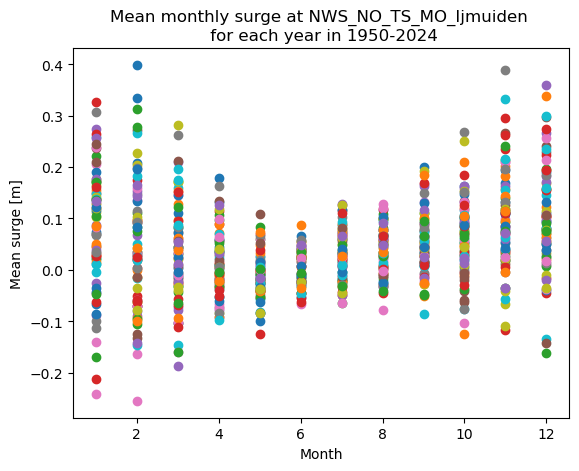
\includegraphics[keepaspectratio]{images/GTSM_monthly_means.png}}

}

\caption{Maandgemiddelde windopzet voor alle jaren over de periode 1950
- 2024. Zie tekst voor meer uitleg.}

\end{figure}%

De correctie voor windopzet wordt als volgt berekend:

\begin{itemize}
\item
  Windopzet wordt gemiddeld per jaar en station
\item
  Jaargemiddelde windopzet wordt getransformeerd tot jaarlijkse
  afwijking (opzetanomalie) van het gemiddelde
\item
  De opzetanomalie per jaar en station wordt afgetrokken van de
  zeespiegelhoogte om tot de gecorrigeerde zeespiegel te komen
\end{itemize}

Voor het gemiddelde over Nederland worden de gecorrigeerde
zeespiegelwaarden gemiddeld over de stations.

De huidige versie van GTSM die gebruikt wordt voor berekening van
windopzet voor de Zeespiegelmonitor wordt aangestuurd door een waterpeil
inclusief een stijging. De zeespiegelstijging die is toegepast is
afgeleid van SLR-projecties in Fifth Assessment Report IPCC (AR5) van
Intergovernmental Panel on Climate Change (IPCC). Deze wijken
waarschijnlijk af van de daadwerkelijk waargenomen zeespiegelstijging.
Het is daarom belangrijk om te weten of de gebruikte stijging invloed
heeft op de berekende windopzet aan de Nederlandse kust. Dit is
gecontroleerd door de GTSM-ERA5 modelopstelling voor 2023 te draaien,
zodat modelresultaten zowel met als zonder Sea Level Rise (SLR) (totaal
waterpeil en alleen getijdenruns) worden getoond. Deze resultaten zijn
vergeleken (zoals te zien in dit
\href{https://github.com/VU-IVM/gtsm3-era5-nrt/blob/main/02_analysis_and_validation/p06_compare_SLR_effect_surge_mean.ipynb}{rekendocument}.

Uit deze resultaten kan worden geconcludeerd:

\begin{itemize}
\tightlist
\item
  SLR in 2023, die in onze modelruns is opgenomen, is \textasciitilde0,1
  m. \textbf{!! Ten opzichte van welk jaar? !!}
\item
  Dit niveau van SLR heeft geen significant effect op de gemiddelde
  windopzet. Het verschil dat het model veroorzaakt is verwaarloosbaar
  (minder dan 1 mm).
\item
  Op enkele locaties diep in de Waddenzee is er enig verschil in
  windopzet tussen de twee runs, maar dit zijn locaties in relatief
  afgesloten gebieden in ondiep water. Het verschil blijft beperkt tot
  enkele millimeters ().
\end{itemize}

\begin{figure}[H]

{\centering \pandocbounded{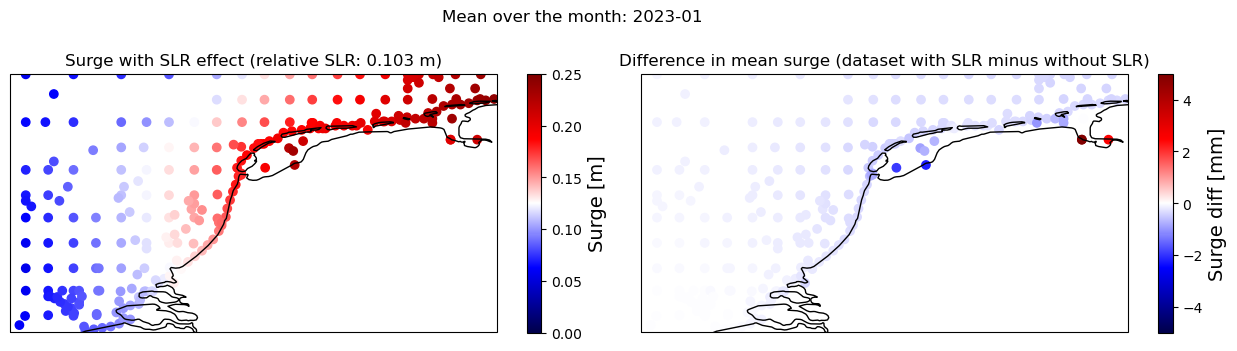
\includegraphics[keepaspectratio]{images/GTSM_SLR_diff.png}}

}

\caption{Gemiddelde windopzet op de zeespiegel voor 2023 inclusief
zeespiegelstijging zoals gedefinieerd in GTSM (linker figuur) en het
verschil in windopzet tussen modelruns met en zonder zeespiegelstijging
(rechter figuur). Voor verder uitleg zie de tekst.}

\end{figure}%

Hieruit concluderen we dat de windopzet uit GTSM inclusief
zeespiegelstijging, die we op dit moment gebruiken voor de
Zeespiegelmonitor, niet wordt beïnvloed door de gebruikte
zeespiegelprojectie. Het verdient wel aanbeveling om in de toekomst GTSM
ook zonder SLR en/of met de gemeten /acr\{SLR\} te laten rekenen.

\section{Getij}\label{getij}

Naast windopzet zorgt ook het getij, met name de nodale cyclus, voor een
variatie in de zeespiegel over de jaren
\citep[\citet{Baart2012}]{Woodworth2012}. Daarom wordt de variatie door
de nodale cyclus meegenomen als gelinearizeerde amplitude en fase, in de
vorm van een u en v component (vergelijking (2.2)). Het is ook mogelijk
om het equilibrium getij (Fedor Baart, van Gelder, et al.~2012) op te
leggen. Het equilibrium getij is het getij dat zou optreden zonder
invloed van land of ondiepte op de propagatie van de getijgolf. In
Nederland en op veel andere plaatsen is de amplitude en fase van het in
de regressie meegenomen nodaal getij niet hetzelfde als het equilibrium
getij. Er is lange tijd discussie geweest over welk getij het meest
geschikt is om mee te rekenen in langjarige analyses (Woodworth vs
Baart). Recent is aangetoond dat het waargenomen nodaal getij aan de
Nederlandse kust verklaarbaar beïnvloed wordt door modulatie van de M2
getijgolf in de Noordzee (Lebars et al., ). Dit brengt de twee
denkbeelden dichter bij elkaar. Het lijkt er hierbij op dat de in de
regressie geschatte nodale cyclus min of meer precies beantwoord aan het
beeld van een gemoduleerd M2 getij.

\section{Rekenmethode voor de bepaling van de huidige
zeespiegelstijging}\label{rekenmethode-voor-de-bepaling-van-de-huidige-zeespiegelstijging}

De stijging van de zeespiegel wordt wiskundig beschreven met een model,
waaruit we de meest waarschijnlijk stijging berekenen over de gewenste
periode (laatste 15 jaar). De keuze van het model dient ook te voldoen
aan de gestelde criteria (\#afwegingen). De keus aan modellen die getest
worden is over de jaren langzaam uitgebreid. In @Dillingh2010 werd een
kwadratische term toegevoegd aan het initiële lineaire model, om een
versnelling al dan niet te accepteren. Er was toen alleen voor station
Den Helder een significante toename van de zeespiegestijging met het
gebruikte model. In de Zeespiegelmonitor 2014 (@Baart2014a) is daarom
alleen het lineaire model toegepast, met een uitbreiding van een LOESS
term om het model beter te laten aansluiten bij projecties. In de
Zeespiegel 2018 (@Baart2019) is opnieuw de kwadratische term als
toevoeging op het lineaire model getest, samen met een trendbreuk model
(gebroken lineair model) waarbij het breekpunt in 1993 gekozen werd. De
keuze voor 1993 was gemotiveerd door:

\begin{itemize}
\tightlist
\item
  1993 is het startjaar van satellietmetingen. Door de breuk in 1993 te
  leggen wordt de trend ook berekend vanaf dit jaar, wat vergelijking
  met satellietmetingen vergemakkelijkt. Tevens wordt de aansluiting met
  gegevens van vóór 1993 behouden.
\item
  Rond 1993 stond de zeespiegel vrij laag, deels door de uitbraak van de
  Pinatubo vulkaan. Gedeeltelijk daardoor laten latere analyses zien dat
  voor een gebroken lineair model dit het meest waarschijnlijke
  breekpunt is {[}@{]}.
\end{itemize}

\section{Metingen van het zeeniveau met satellieten
(altimetrie)}\label{altimetrie}

uitleg, voordelen, nadelen, verschillen. Zie ook eerdere rapportages.

\subsection{Beschikbare satellieten en
metingen}\label{beschikbare-satellieten-en-metingen}

\subsection{Nieuwe satellieten}\label{nieuwe-satellieten}

\subsection{Wanneer kan overgegaan worden op
satellietmetingen}\label{wanneer-kan-overgegaan-worden-op-satellietmetingen}

\bookmarksetup{startatroot}

\chapter{Resultaten}\label{resultaten}

\section{Voorkeursmodel}\label{voorkeursmodel}

\section{Huidige zeespiegel(stijging)}\label{huidige}

\section{Bodemdaling en
zeespiegelstijging}\label{bodemdaling-en-zeespiegelstijging}

Bij alle getijdenstations bestaat het gemeten relatieve
zeespiegelstijgingssignaal voor een deel uit lange-termijn geologische
bodemdaling \citep{Hijma2025b}. Deze daling wordt hoofdzakelijk
veroorzaakt door tektonische en glacio-isostatische bodemdaling en heeft
dalingssnelheden die van zuid naar noord toenemen van circa 2 naar 5
cm/eeuw (Figure~\ref{fig-totgeol100yr}). De metingen worden hier niet
voor gecorrigeerd en de via PSMSL beschikbare zeespiegeldata omvatten
dus deze lange-termijn geologische bodemdalingscomponent.

\begin{figure}

\centering{

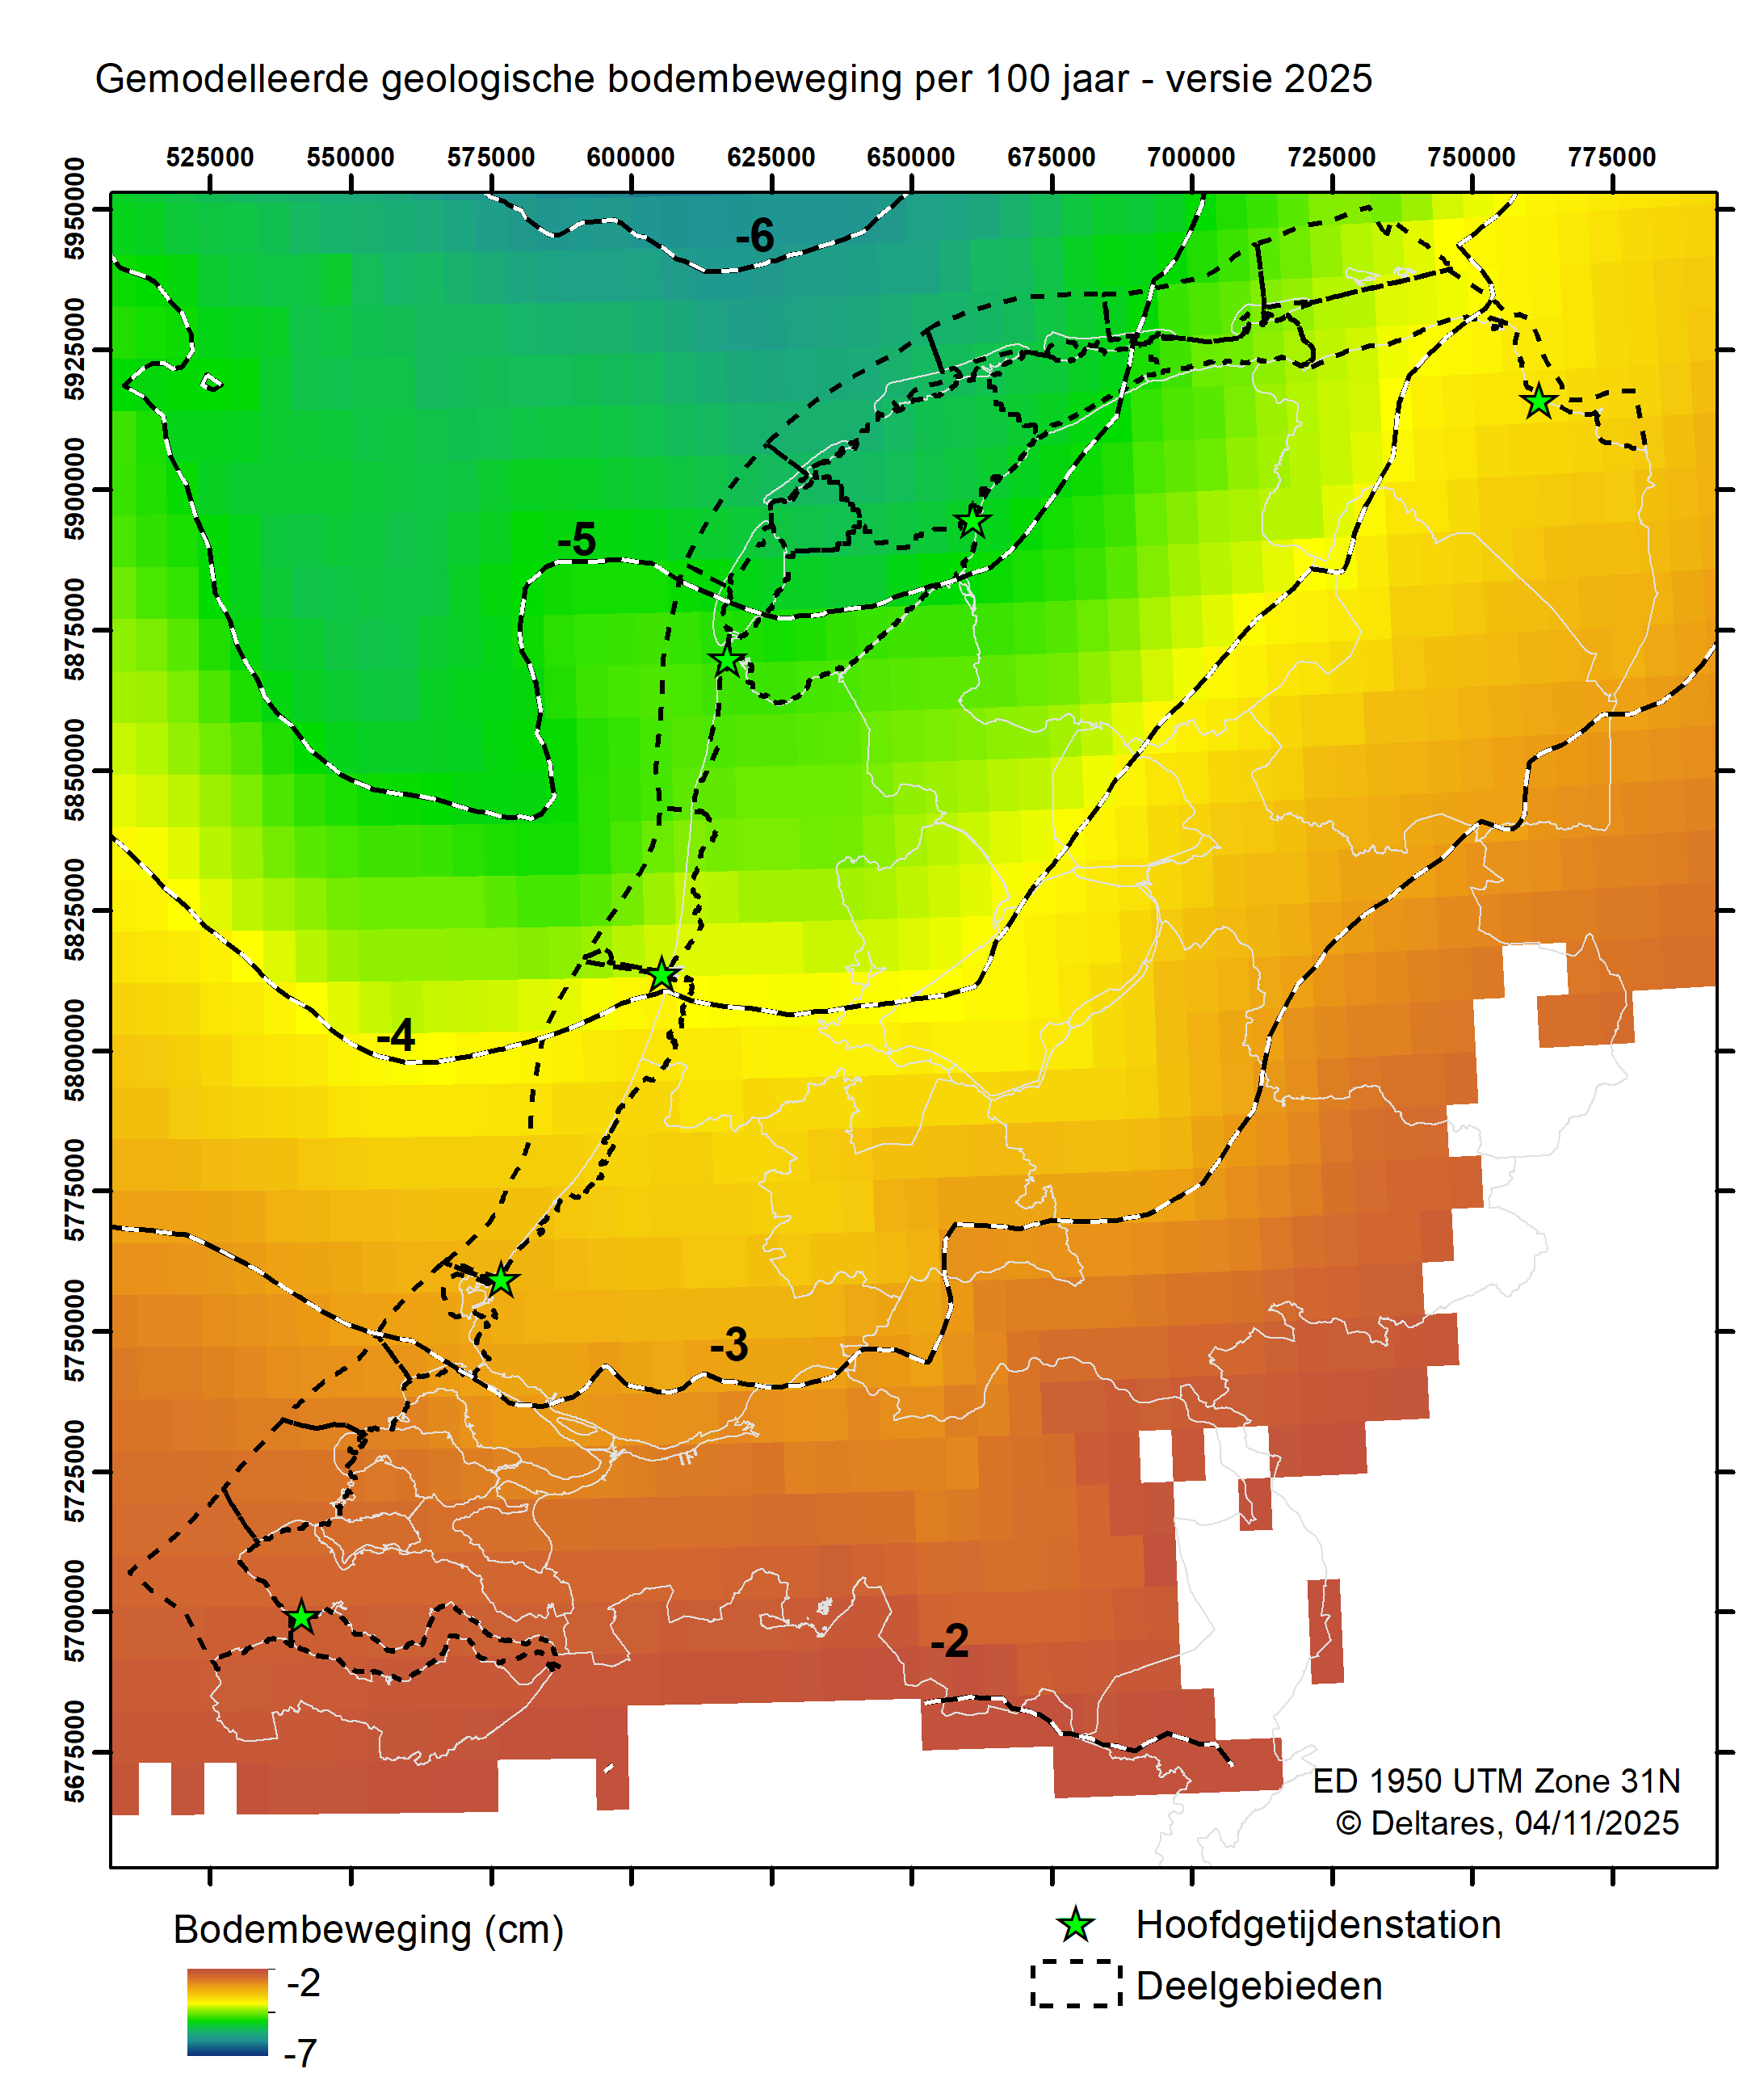
\includegraphics[width=0.8\linewidth,height=\textheight,keepaspectratio]{images/Totgeol100yr_nieuw.png}

}

\caption{\label{fig-totgeol100yr}Geologische bodemdaling per 100 jaar
\citep{Hijma2025b}}

\end{figure}%

Er zijn twee stations waar ook bodemdaling door gaswinning heeft
plaatsgevonden, namelijk Hoek van Holland en Delfzijl. Bij Hoek van
Holland gaat het om 1-2 cm in de laatste decennia en gaan we er vanuit
dat deze daling in het zeespiegelsignaal zit. De verwachte daling door
gaswinning in de komende decennia is minder dan 1 cm \citep{Hijma2026}.
De daling bij Delfzijl is veel groter geweest en bedraagt ongeveer 30 cm
sinds 1963. Voor Delfzijl weten we vrij zeker dat de bodemdaling sinds
1973 niet in de zeespiegeldata zit, maar dat de metingen gecorrigeerd
worden \citep[punt 5]{Jong1973}. Dit betekent dat de relatieve
zeespiegelstijging bij Delfzijl eigenlijk sneller gaat dan in PSMSL
gepubliceerd wordt, omdat de daling door gaswinning niet meegenomen
wordt. Tussen de start van de gaswinning in Groningen in 1963 en 1973
daalde de bodem bij Delfzijl ongeveer 7 cm. Wij gaan er hier vanuit dat
deze daling op dezelfde manier is behandeld als de daling na 1973,
conform \citep[punt 5]{Jong1973}, en dus niet in het zeespiegelsignaal
zit. Door het dichtdraaien van de gaskraan is de daling bij het station
sterk afgenomen en naar verwachting zal deze nog slechts enkele
centimeters bedragen in de komende decennia \citep{Hijma2026}.

In de toekomst zal station Harlingen waarschijnlijk beïnvloed gaan
worden door bodemdaling door zoutwinning. De winning is recent gestart
in de Waddenzee ten westen van Harlingen en de bodemdalingsschotel lijkt
Harlingen op termijn te gaan bereiken. Dit zal de komende 30 jaar tot
meerdere centimeters bodemdaling leiden \citep{Hijma2025c, Hijma2026}.
De onzekerheid is echter groot en een kleine verschuiving in de vorm of
positie van de schotel kan resulteren in geen extra bodemdaling of juist
nog enkele centimeters meer. De extra bodemdaling wordt gelukkig
gemonitord, waardoor een eventuele impact op de zeespiegelmetingen goed
in beeld zal komen.

Bij de meeste stations is de totale bodemdaling dus gelijk aan de
geologische bodemdaling, maar bij enkele stations is de totale
bodemdaling een optelsom van de geologische bodemdaling en de daling
door delfstofwinning. Table~\ref{tbl-bodemdalingscomponenten} geeft per
station de verschillende bodemdalingscomponenten, de gemeten relatieve
zeespiegelstijging en de afgeleide absolute zeespiegelstijging.

\begin{longtable}[]{@{}
  >{\raggedright\arraybackslash}p{(\linewidth - 10\tabcolsep) * \real{0.1667}}
  >{\raggedright\arraybackslash}p{(\linewidth - 10\tabcolsep) * \real{0.1667}}
  >{\raggedright\arraybackslash}p{(\linewidth - 10\tabcolsep) * \real{0.1667}}
  >{\raggedright\arraybackslash}p{(\linewidth - 10\tabcolsep) * \real{0.1667}}
  >{\raggedright\arraybackslash}p{(\linewidth - 10\tabcolsep) * \real{0.1667}}
  >{\raggedright\arraybackslash}p{(\linewidth - 10\tabcolsep) * \real{0.1667}}@{}}
\caption{Uitsplitsing bodemdaling \citep[op basis van][ and
\citet{Hijma2026}]{Hijma2025b} en zeespiegelstijging per station (dit
rapport). Geologische bodemdaling is constant op tijdschalen van eeuwen,
de dalingssnelheid door winning is berekend voor de periode 1997-2026.
De totale bodemdaling bij Hoek van Holland is inclusief daling door
winning, bij Delfzijl exclusief daling door winning (zie tekst). De
gemiddelde relatieve zeespiegelstijging is gemeten over de periode xxx
(gebroken lineair
model).}\label{tbl-bodemdalingscomponenten}\tabularnewline
\toprule\noalign{}
\begin{minipage}[b]{\linewidth}\raggedright
station
\end{minipage} & \begin{minipage}[b]{\linewidth}\raggedright
Geologische bodemdaling (mm/jaar)
\end{minipage} & \begin{minipage}[b]{\linewidth}\raggedright
Daling door winning (mm/jaar)
\end{minipage} & \begin{minipage}[b]{\linewidth}\raggedright
Totale bodemdaling (mm/jaar)
\end{minipage} & \begin{minipage}[b]{\linewidth}\raggedright
Huidige relatieve ZSS (mm/jaar)
\end{minipage} & \begin{minipage}[b]{\linewidth}\raggedright
Huidige absolute ZSS (mm/jaar)
\end{minipage} \\
\midrule\noalign{}
\endfirsthead
\toprule\noalign{}
\begin{minipage}[b]{\linewidth}\raggedright
station
\end{minipage} & \begin{minipage}[b]{\linewidth}\raggedright
Geologische bodemdaling (mm/jaar)
\end{minipage} & \begin{minipage}[b]{\linewidth}\raggedright
Daling door winning (mm/jaar)
\end{minipage} & \begin{minipage}[b]{\linewidth}\raggedright
Totale bodemdaling (mm/jaar)
\end{minipage} & \begin{minipage}[b]{\linewidth}\raggedright
Huidige relatieve ZSS (mm/jaar)
\end{minipage} & \begin{minipage}[b]{\linewidth}\raggedright
Huidige absolute ZSS (mm/jaar)
\end{minipage} \\
\midrule\noalign{}
\endhead
\bottomrule\noalign{}
\endlastfoot
Vlissingen & 0.23 & 0 & 0.23 & ??? & ???? \\
Hoek van Holland & 0.33 & 0.2 & 0.53 & ??? & ??? \\
IJmuiden & 0.42 & 0 & 0.42 & ??? & ??? \\
Den Helder & 0.48 & 0 & 0.48 & ??? & ??? \\
Harlingen & 0.37 & 0 & 0.37 & ??? & ??? \\
Delfzijl & 0.39 & 4 & 0.39 & ??? & ??? \\
\end{longtable}

\section{Vergelijking met scenarios
(KNMI)}\label{vergelijking-met-scenarios-knmi}

\section{Vergelijking met
zeespiegelbudgetten}\label{vergelijking-met-zeespiegelbudgetten}

\section{Variatie binnen Nederland}\label{variatie-binnen-nederland}

\section{Vergelijking? met
satellietmetingen}\label{vergelijking-met-satellietmetingen}

\bookmarksetup{startatroot}

\chapter{Discussie}\label{discussie}

\section{Toepassingsbereik van de gebruikte
methodiek}\label{toepassingsbereik}

\section{Vergelijking met andere methoden om zeespiegelstijging vast te
stellen}\label{zss-vergelijking}

(KNMI, Staatstoezicht op de mijnen, TNO, PBL)

\section{Verschillen binnen Nederland
\{verschillen-binnen-nederland\}}\label{verschillen-binnen-nederland-verschillen-binnen-nederland}

\bookmarksetup{startatroot}

\chapter*{Literatuur}\label{literatuur}
\addcontentsline{toc}{chapter}{Literatuur}

\markboth{Literatuur}{Literatuur}

\renewcommand{\bibsection}{}
\bibliography{bib/literatuurWillemMod.bib,bib/sealevel.bib}

\bookmarksetup{startatroot}

\chapter*{Bijlagen}\label{bijlagen}
\addcontentsline{toc}{chapter}{Bijlagen}

\markboth{Bijlagen}{Bijlagen}

\section*{Bodemdaling}\label{bodemdaling}
\addcontentsline{toc}{section}{Bodemdaling}

\markright{Bodemdaling}

Het is al heel lang bekend dat de zeespiegelmetingen in Nederland worden
beïnvloed door bodemdaling \citep[\citet{Veen1954}]{Veen1945} en dat ze
feitelijk de relatieve zeespiegelbewegingen weergeven. Bodemdaling is de
optelsom van verschillende componenten
(Figure~\ref{fig-Bodemdalingscomponenten}) en niet alle componenten zijn
relevant voor de zeespiegelmetingen. Dit komt omdat de stations diep
gefundeerd staan en alleen beïnvloed worden door bodemdaling in de lagen
onder de fundering. Maaivelddaling door veenoxidatie of verlaging van de
grondwaterstand hebben dus geen inlvoed op de zeespiegelmetingen, maar
diepere bodemdaling door geologische processen of gaswinning wel. In
Table~\ref{tbl-bodemdalingscomponenten_uitleg} worden de verschillende
componenten nader omschreven.

\begin{figure}

\centering{

\pandocbounded{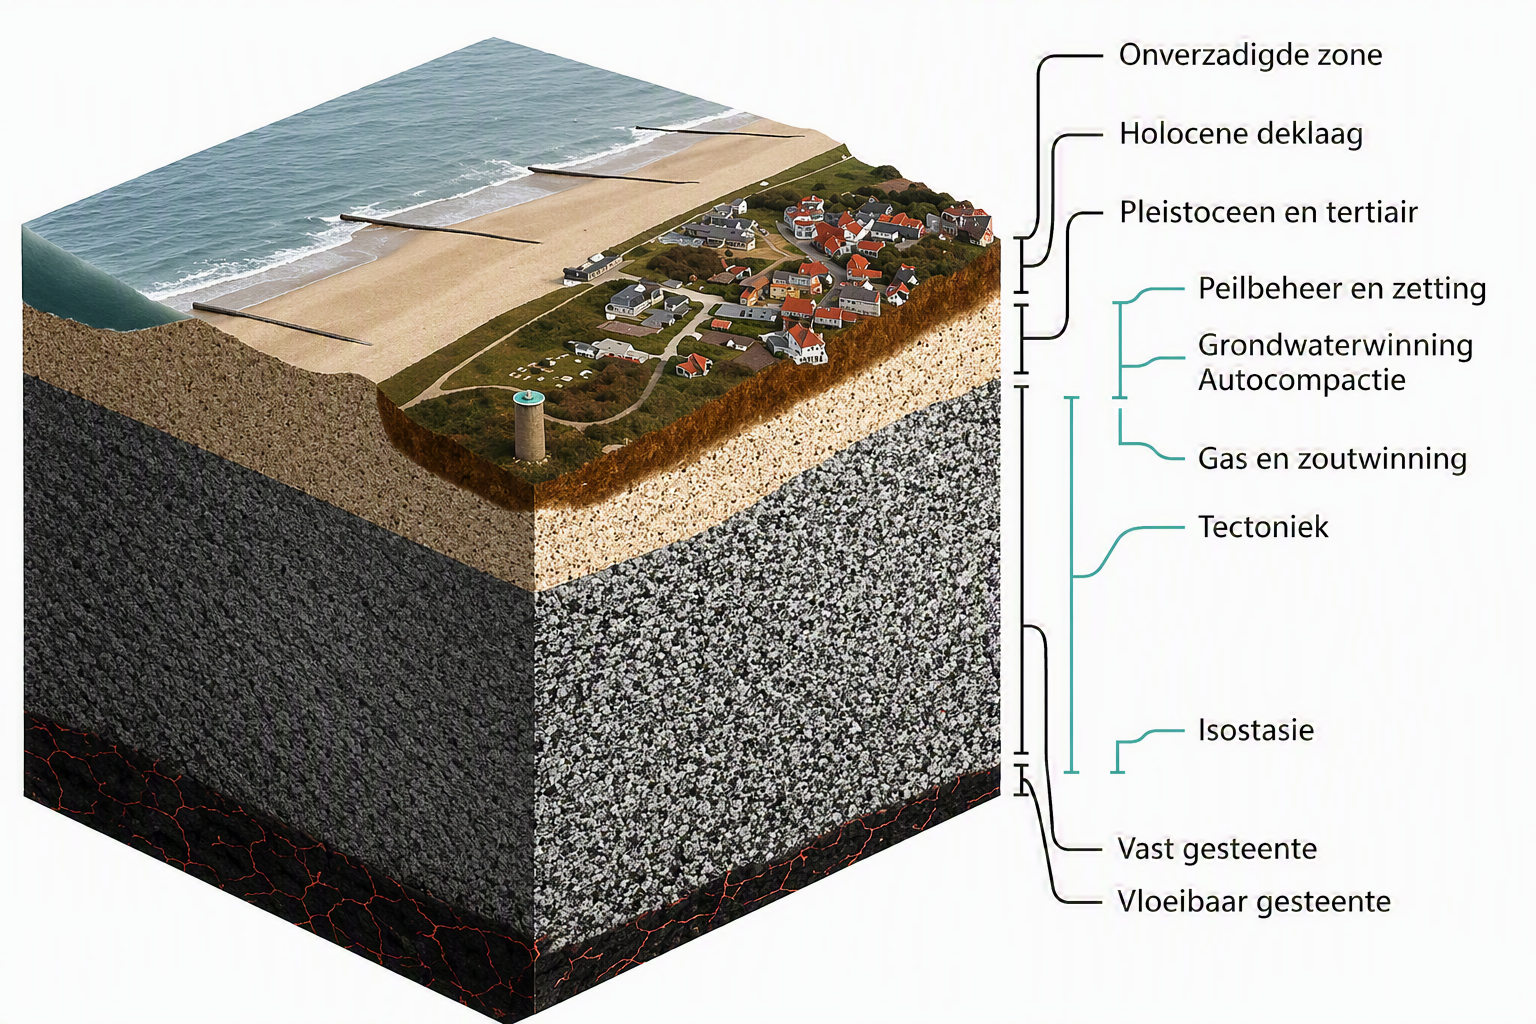
\includegraphics[keepaspectratio]{images/Bodemdalingscomponenten.png}}

}

\caption{\label{fig-Bodemdalingscomponenten}Lagen van de bodem en
componenten van bodemdaling langs de Nederlandse kust. De zwarte lijnen
geven de verschillende ondergrondlagen aan, de blauwgroene lijnen de
bodemdalingscomponenten.}

\end{figure}%

\begin{longtable}[]{@{}
  >{\raggedright\arraybackslash}p{(\linewidth - 4\tabcolsep) * \real{0.3333}}
  >{\raggedright\arraybackslash}p{(\linewidth - 4\tabcolsep) * \real{0.3333}}
  >{\raggedright\arraybackslash}p{(\linewidth - 4\tabcolsep) * \real{0.3333}}@{}}
\caption{De belangrijkste componenten van bodembeweging in Nederland,
afgeleid van \citep[ and
\citet{Hijma2018}]{Hijma2017}.}\label{tbl-bodemdalingscomponenten_uitleg}\tabularnewline
\toprule\noalign{}
\begin{minipage}[b]{\linewidth}\raggedright
Hoofdoorzaak
\end{minipage} & \begin{minipage}[b]{\linewidth}\raggedright
Oorzaak
\end{minipage} & \begin{minipage}[b]{\linewidth}\raggedright
Beschrijving
\end{minipage} \\
\midrule\noalign{}
\endfirsthead
\toprule\noalign{}
\begin{minipage}[b]{\linewidth}\raggedright
Hoofdoorzaak
\end{minipage} & \begin{minipage}[b]{\linewidth}\raggedright
Oorzaak
\end{minipage} & \begin{minipage}[b]{\linewidth}\raggedright
Beschrijving
\end{minipage} \\
\midrule\noalign{}
\endhead
\bottomrule\noalign{}
\endlastfoot
Geologische bodembeweging & Tektoniek (0.2-1.5 cm/eeuw & Daling of
opheffing die wordt veroorzaakt door spanningen in de ca. 100 km dikke
Euraziatische aardplaat waar Nederland deel van uitmaakt. De spanningen
hangen samen met het naar elkaar toe bewegen van de Afrikaanse en
Euraziatische aardplaat en het uit elkaar drijven van Europa en
Noord-Amerika. De snelheid van tektonische bodemdaling neemt toe van
Goeree (2 mm/eeuw) tot meer dan 1 cm/eeuw in de Waddenzee. \\
Geologische bodembeweging & Isostasie(2-5 cm/eeuw) & Daling die
samenhangt met het terugbuigen van de aardplaat in Noordwest Europa door
het afsmelten van de grote ijskappen die in de laatste glaciale periode
op Groot-Brittannië en Scandinavië rustten. Bij het ontstaan van de
ijskappen werd de aardplaat onder het gewicht van het vele ijs
doorgebogen en in een rand daarom heen kwam de aardplaat juist omhoog.
Het proces van herstel (terugbuigen) is nog gaande, en omdat Nederland
op de omhoogkomende rand lag daalt Nederland. \\
Geologische bodembeweging & Autocompactie (\textless\textless{} 1
cm/eeuw) & Samendrukking van afzettingen tussen het maaiveld en
honderden meters diepte. Deze compactie vindt \\
plaats onder het eigen gewicht en door toename van dat gewicht in het
recente geologische verleden door jonge afzettingen. & & \\
Antropogene bodemdaling & Olie-/gaswinning(cm-dm per eeuw) & Daling aan
het maaiveld die wordt veroorzaakt door de drukverlaging in olie- of
gasvelden en die zorgt voor samendrukking van de betreffende lagen.
Speelt bij Hoek van Holland en Delfzijl. \\
Antropogene bodemdaling & Zoutwinning (cm-m per eeuw) & Daling die wordt
veroorzaakt door de lage druk in de cavernes die ontstaan door het
winnen van zout. De cavernes worden langzaam dichtgedrukt en zorgen voor
inzakking van bovenliggende lagen. Speelt mogelijk over enige tijd bij
Harlingen. \\
Antropogene bodemdaling & Grondwaterwinning (cm-dm per eeuw) & Daling
die wordt veroorzaakt door de waterdrukverlaging in de bodemlagen in de
omgeving van de winning waardoor de laag waaruit wordt gewonnen, maar
ook boven en/of onderliggende lagen, worden samengedrukt. \\
Antropogene bodemdaling & Peilbeheer (cm-dm per eeuw) & Daling die
samenhangt met periodische aanpassing/verlaging (t.o.v. NAP) van het
waterpeil in sloten \\
en vaarten in gebieden met maaivelddaling om een gewenste drooglegging
(verschil tussen maaiveld en waterpeil) te handhaven. & & \\
Antropogene bodemdaling & Zetting (cm-dm per eeuw) & Daling onder
invloed van extra gewicht dat op het maaiveld (of waterbodem) wordt
aangebracht door de mens en waardoor lagen in de ondergrond worden
samengedrukt. \\
\end{longtable}

%------------------------------------------------------------------------------
\end{document}
